\iffalse
\documentclass{article}
\usepackage{amsmath, amssymb, amsfonts, amsthm}
\usepackage{enumitem}
\usepackage{tabularx}
\usepackage{lipsum}
\usepackage{xcolor}
\usepackage{float}
\usepackage{ragged2e}
\usepackage{titlesec}
\usepackage{graphicx}
\usepackage{watermark}
\usepackage{hyperref,xcolor}
\usepackage{commath}
\usepackage{gensymb}
\usepackage{array}
\usepackage{amsmath}
\usepackage{listings}
\usepackage[e]{esvect}
\graphicspath{ {./sdcard/Download/fwc/} }
%\newcommand{\myvec}[2][1mu]{\vec{#2\mkern-#1}\mkern#1}
\newcommand{\myvec}[1]{\ensuremath{\begin{pmatrix}
#1\end{pmatrix}}}
\hypersetup{
	colorlinks,
	urlcolor={black}%black!50!blue
}
\providecommand{\mtx}[1]{\mathbf{#1}}
\newcommand{\Mod}[1]{\(\mathrm{mod}\#1)}
\let\vec\mathbf
\providecommand{\cbrak}[1]{\ensuremath{\left\{#1\right\}}}
\newcommand{\Problem}{\noindent \teextbf{Problem:}}
\newcommand{\solution}{\noindent \teextbf{Solution:}}
\setlist[enumerate]{font=\small\bfseries}
\newcommand{\figuremacro}[5]{
	}
\lstset{
	frame=single,
	breaklines=true,
	columns=fullflexible
	}

\begin{document}

\begin{center}
	\color{blue} CHAPTER 7: TRIANGLES
\end{center}
\begin{center}
	\color{blue} EXERCISE 7.3
\end{center}
\fi

\begin{enumerate}[label=\thesection.\arabic*,ref=\thesection.\theenumi]
	\item $\vec{ABC}$ is an isosceles triangle with $\vec{AB=AC}$ and $\vec{BD}$ and $\vec{CE}$ are its two medians. Show that $\vec{BD=CE}$.
	\item In Fig. \ref{fig:exemplar/9.7.37.3.2}, $\vec{D}$ and $\vec{E}$ are the points on side $\vec{BC}$ of a $\triangle \vec{ABC}$ such that $\vec{BD=CE}$ and $\vec{AD=AE}$. Show that $\triangle \vec{ABD} \cong \triangle \vec{ACE}$.
\begin{figure}[h]
	\centering
	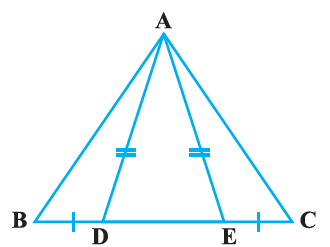
\includegraphics[width=\columnwidth]{exemplar/9.7.3/figs/Figure1.png}
	\caption{}
	\label{fig:exemplar/9.7.37.3.2}
\end{figure}
\item $\vec{CDE}$ is an equilateral triangle formed on a side $\vec{CD}$ of a square $\vec{ABCD}$ (Fig. \ref{fig:exemplar/9.7.37.3.3}). Show that $\triangle \vec{ADE} \cong \triangle \vec{BCE}$.
\begin{figure}[h]
	\centering
	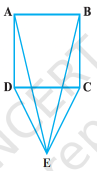
\includegraphics[width=\columnwidth]{exemplar/9.7.3/figs/Figure2.png}
	\caption{}
	\label{fig:exemplar/9.7.37.3.3}
\end{figure}
\item In Fig. \ref{fig:exemplar/9.7.37.3.4}, $\vec{BA} \perp \vec{AC}$, $\vec{DE} \perp \vec{DF}$ such that $\vec{BA=DE}$ and $\vec{BF=EC}$. Show that $\triangle \vec{ABC} \cong \triangle \vec{DEF}$.
\begin{figure}[h]
	\centering
	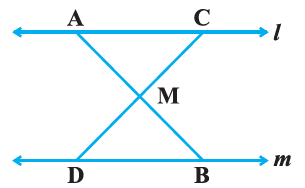
\includegraphics[width=\columnwidth]{exemplar/9.7.3/figs/Figure3.png}
	\caption{}
	\label{fig:exemplar/9.7.37.3.4}
\end{figure}
\item $\vec{Q}$ is a point on the side $\vec{SR}$ of $\triangle \vec{PSR}$ such that $\vec{PQ=PR}$. Prove that $\vec{PS>PQ}$.
\item $\vec{S}$ is any point on side $\vec{QR}$ of a $\triangle \vec{PQR}$. Show that $\vec{PQ+QR+RP>2PS}$.
\item $\vec{D}$ is any point on side $\vec{AC}$ of a $\triangle \vec{ABC}$ with $\vec{AB=AC}$. Show that $\vec{CD<BD}$.
\item In Fig. \ref{fig:exemplar/9.7.37.3.8}, $\vec{l} \| \vec{m}$ an $\vec{M}$ is the mid-point of a line segment $\vec{AB}$. Show that $\vec{M}$ is also the mid-point of any line segment $\vec{CD}$, having its end points on $\vec{l}$ and $\vec{m}$, respectively.
\begin{figure}[h]
	\centering
	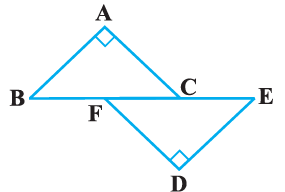
\includegraphics[width=\columnwidth]{exemplar/9.7.3/figs/Figure4.png}
	\caption{}
	\label{fig:exemplar/9.7.37.3.8}
\end{figure}
\item Bisectors of the $\angle \vec{B}$ and $\angle \vec{C}$ of an isosceles triangle with $\vec{AB=AC}$ intersect each other at $\vec{O}$. $\vec{BO}$ is produced to a point $\vec{M}$. Prove that $\angle \vec{MOC}= \angle \vec{ABC}$.
\item Bisectors of the $\angle \vec{B}$ and $\angle \vec{C}$ of an isosceles triangle $\vec{ABC}$ with $\vec{AB=AC}$ intersect each other at $\vec{O}$. Show that the external angle adjacent to $\angle \vec{ABC}$ is equal to $\angle \vec{BOC}$.
\item In Fig. \ref{fig:exemplar/9.7.37.3.11}, $\vec{AD}$ is the bisector of $\angle \vec{BAC}$. Prove that $\vec{AB>BD}$.
\begin{figure}[h]
	\centering
	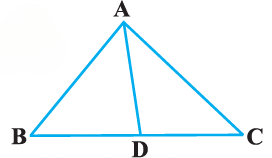
\includegraphics[width=\columnwidth]{exemplar/9.7.3/figs/Figure5.png}
	\caption{}
	\label{fig:exemplar/9.7.37.3.11}
\end{figure}
\end{enumerate}
